\section{(Journal version) NP-completeness of RS(2)+MA(4)+FP}

\subsection{Intro}

\begin{enumerate}
  \item Needed properties: FP, RS(2), MA(4)
  \item Eliminated any need for bandwidth constraints, node interconnect and idle machines
\end{enumerate}

\subsection{Notation}

(3DPM) We call $deg(e)$ the number of triples that contain element
$e\in A\cup B\cup C$. We call $n=|A|$; please note that
$n=|A|=|B|=|C|$. We call $t$ the number of triples. We call $t(e)$ the
set of triples containing element $e$. We call
$\lbrace e_1(t), e_2(t), e_3(t) \rbrace$ the elements of triple $t$. We call $m$ the number of triples.

\subsection{The construction}

\begin{figure}[t]
\centering
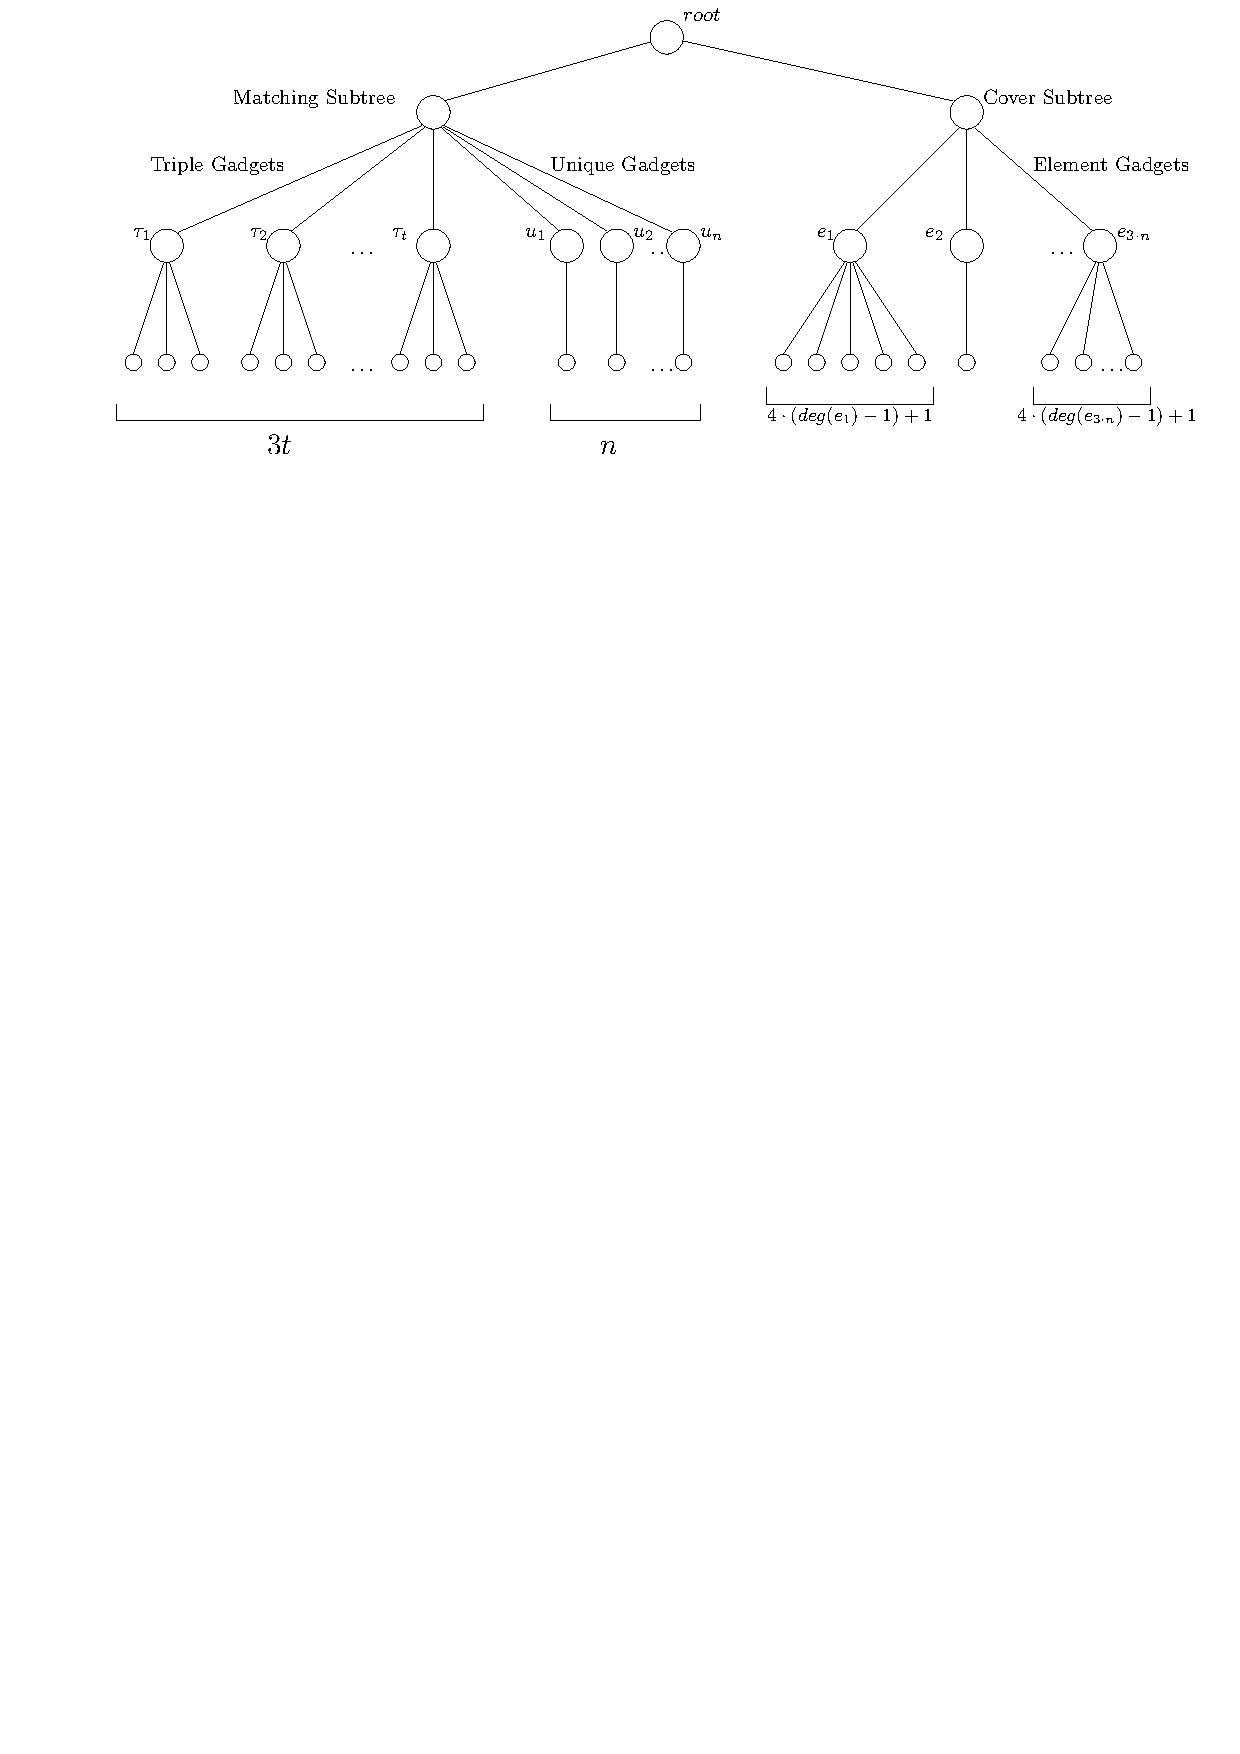
\includegraphics[width=0.99\columnwidth]{reduction/overview.pdf}
\vspace{-1em}
\caption{Overview of the substrate network}
\vspace{-1em}
\end{figure}


Let's take any instance $I$ of 3D Perfect Matching and create a VCEMB
instance $I'$ in the following way:

(chunk types) We construct the following chunk types:
\begin{itemize}
\item for each element $e\in A\cup B\cup C$ we construct $deg(e)$
  chunk types. We will refer to such chunk types in two ways: either
  the element of set $t(e)$ for some element $e$, or $e_i(t)$ for some
  triple $t$ and index $i \in \{1,2,3\}$
\item we construct $n$ chunk types named $u_1, \ldots, u_n$ (intuitions: we want to choose $n$ triples to our solution)
\item (unique chunks) again, for each element $e\in A\cup B\cup C$ we construct additional $3\cdot(deg(e) - 1)$ chunks. We call this set $U(e)$.
\end{itemize}

(tree) 

\begin{enumerate}
%\item (chunk types) There are the following chunk types: (1) For each
%  element $e \in A\cup B\cup C$ we create $4\cdot deg(e)$ chunk types,
%  where $a\in{0,1,2}$ is to make $deg(e)-1+a$ divisible by 3. We those
%  chunk types $core(e)$ (both corresponding to degree and those
%  additional).
%\item (unique chunk types) We create additional chunk types which will
%  have only one replica. We create $n$ chunk types and we call this
%  set $mtch$. For each element $e\in A\cup B\cup C$ we create
%  $core(e)/3$ chunk types called $unqCore(e)$.
%\item (convention for core chunk types naming) Let's say that $e$ is
%  in triples $t_1,t_2,\ldots,t_{deg(e)}$; then
%  $core(e) = \{ e^{t_1}, e^{t_2}, \ldots, e^{t_{deg(e)}} \} \cup
%  ADDITIONAL$,
%  where $ADDITIONAL$ are the chunk types that were added to make
%  $deg(e)-1+a$ divisible by 3.
\item (tree) physical network consists of two parts: Matching Subtree
  and Cover Subtree. Matching Subtree consists of two parts: $t$
  Triple Gadgets and Unique Gadgets. Cover Subtree consists of
  $n$ Element Gadgets.
\item (Triple Gadget) For each triple we create a subtree
  consisisting of 4 vertices: three leaves and one root of the
  triple. We attach the root of the triple to root of Matching
  Subtree.
\item (Unique Gadget) We create $1$ leaf and $1$ middle node and
  connect it to the root of Matching Subtree. Note that we create middle
  nodes not only to keep the tree balanced, but also to keep leaves of
  Unique Gadgets far from leaves of other Unique Gadgets.
\item (Element Gadget) For each element $e \in A\cup B\cup C$ we
  construct the subtree consisting of a root of the element (attached
  to the root of Cover Subtree), and with $4\cdot(t(e)-1)+1$
  leaves.

\end{enumerate}

(chunk placement)
\begin{enumerate}
\item (chunks in Triples Subtree) For each triple
  $t$ we put three chunks in leaves of
  the corresponding Triple Gadget: $e_1(t), e_2(t), e_3(t)$.
\item (chunks in Unique Subtree) We put chunks $u_1,\ldots, u_n$ in leaves of
  Unique Gadgets.
\item (chunks in Element Gadget) For each element $e\in A\cup B\cup C$ we place chunks
  $t(e)\cup U(e)$ in leaves of each Element Subtree.
\end{enumerate}

(other properties of the instance)
\begin{enumerate}
\item (multiple assignment) We set the number of processed chunks by
  each machine to 4.
\item (number of machines) We allow to spawn
  $numVMs := n + \sum_{e}(deg(e)-1)$ machines.
\item (threshold)
  $Thr := n\cdot (0 + 2 + 2 + 4) + \sum_{e}(deg(e)-1)\cdot (0 + 2 + 2 + 2)$
\end{enumerate}

This ends the construction. The instance produced such way uses two replicas of each chunk type.

\begin{obs}
We have one instance of each chunk type in Matching Subtree.
\end{obs}

\begin{obs}
We have one instance of each chunk type in Elements Subtree.
\end{obs}

\begin{corollary}
We have at most two replicas of each chunk type in the substrate network.
\end{corollary}


\subsection{The reduction -- constructing VCEMB solution from 3DPM
  solution}

\begin{enumerate}
  \item We put $n$ VMs in any leaf of such Triple Subtries that were
  chosen in 3DPM solution. For each such VM we match to it 3 chunks
  that are put in its Triple Gadget (it is sitting on one of them),
  and we match it to any unmatched chunk in any Unique Gadget
  \item We put $deg(e)-1$ VMs in each Element Subtree. We match all remaining
  chunks from this Element Subtree to those VMs in any possible
  way.
  \item Such a solution has cost $\leq Thr$ (easy to see by
  summing costs of transporting chunks to each VM)
  \item Feasibility of the constructed solution: each chunk type was processed. Each VM processes 4 chunks.
\end{enumerate}

\subsection{The reduction -- constructing 3DPM solution from VCEMB
  solution}

\begin{theorem}
  Let's take any feasible solution $S$ to the instance $I$ of VCEMB
  (as constructed above). If cost of $S$ is at most $Thr$, then no VM
  is spawned in Unique Subtree.
  \label{th:no-unique}
\end{theorem}

\begin{proof}
  Let's assume the contrary, that in feasible solution $S$ at least
  one VM spawned in Unique Subtree. We show that in this case, the
  cost of solution $S$ is greater than $Thr$.

  Let's name $l$ the number of VMs that was spawned in $S$ in Unique
  Subtree. We know that $1 \leq l \leq t$. We denote the set of VMs
  spawned in Unique Subtree as $U_{VM}$.

  In $S$ we have exactly $4 \cdot numVMs$ chunk transportations, some
  incurring cost $0, 2, 4$ or $6$ (tree has edge-height of $3$). At
  most $numVMs$ transportations are of cost $0$. Note that leaves of
  Unique Subtree are separated from other leaves of the tree by at
  least $4$ edges.

  Cost of chunk transportation to VM $v \in U_{VM}$ is at least
  $0 + 4 + 4 + 4$. The chunks in Unique Subtree are unique, therefore
  we need to transport $t - l$ chunks to machines outside of the
  Unique Subtree, incurring cost $4$ for each of the chunk.

  We lower-bound the cost of each of remaining transportations as $2$.

  Summing the total cost, we have:

  $cost(S) \geq costEstim(l) = 0 \cdot numVMs + l \cdot 12 +
  (t-l)\cdot 4 + (4\cdot numVMs - numVMs - 4\cdot l - (t-l))\cdot 2$

  It can be verified that for each $l$ we have that
  $costEstim(l) > Thr$. To do so, we first show that
  $costEstim(l+1) \geq costEstim(l)$, for $1\leq l \leq t-1$. We have
  that $cost(S) \geq costEstim(1) \geq Thr$.
\end{proof}

\begin{theorem}
  Let's take any feasible solution $S$ to the instance $I$ of VCEMB
  (as constructed above). If cost of $S$ is at most $Thr$, then
  exactly $n$ VMs spawn in Matching Subtree.
  \label{th:np-balance}
\end{theorem}

\begin{proof}
  Let's assume the contrary, that is that the number of VMs $M_{VM}$
  spawned in the Matching Subtree, and $|M_{VM}| \neq n$. We denote
  $l=|M_{VM}|$. First, we use the theorem \ref{th:no-unique} to
  restrict the placement of VMs in Unique Subtree. Then we consider
  cases:
  \begin{enumerate}
  \item $l \leq n$. In this case there are at least
    $u := 4 \cdot (n-l)$ chunks in the Matching Subtree that are not
    processed in the Matching Subtree, each incurring transportation
    cost of $6$. We lower-bound the cost of $S$ in the following way:

    $cost(S) \geq costEstim2(u) = 0\cdot numVMs + 4\cdot t + (4\cdot
    numVms - numVMs - t)\cdot 2$.

    It can be verified that for each $u$ we have that
    $costEstim2(S) > Thr$. To do so, we first show that
    $costEstim2(u+1) \geq costEstim2(u)$, for $1\leq u \leq n-1$. Then
    we show that $costEstim2(1) \geq Thr$.

  \item More than $n$ VMs spawned in Matching Subtree. In this case we
    use the fact that there are not enough VMs in Cover Subtree, and
    we need to transport over $6$ hops at least 3 unique chunks for
    each VM missing.

  \end{enumerate}
\end{proof}

(construction of the matching problem solution)

Let's take any feasible solution $S$ to the instance described
above. We call the Triple Gadget active, if we have a VM spawned in
any leaf of it. We call VMs in active Triple Gadgets the Active VMs We
construct our matching solution $M_S$ from triples that correspond to
active Triple Gadgets.

\begin{lemma}
  If $S$ is feasible, then $M_S$ is feasible.
\end{lemma}

\begin{proof}
\item Exactly $n$ Triple Gadgets are active (\ref{np-balance}).
\item Note that in $S$ only one VM is spawned in Active Triple Gadget.
\item Each Active VM $v$ processes the 3 chunks that are placed in
  $v$'s Triple Gadget, as well as one chunk in Unique Gadget.
\item Every chunk type was covered
\item In each Element Gadget for element $e$, one chunk instance of
  set $t(e)$ was not processed. Let's call this chunk instance
  $np(e)$. Let's call $np = \cup_e np(e)$. We have that $|np| = n$
\item Set $np$ was covered by Active VMs
\item
\end{proof}

\section{(Journal version) NP-completeness of RS(2)+NI+BW+FP}

\subsection{The construction}

\begin{enumerate}
\item the network is reduced network from previous proof (no Unique Subtree, no unique chunks in Elements Subtree)
\item Chunks are placed the same way, with an exception that we have no unique chunk types
\item Set the bandwidth: at most 3 machines i
\item TODO: Description of the construction in NI proof
\item TODO: Proof the lemmas in MA proof
\item TODO: Formulate and proof the bandwidth lemma in NI proof
\end{enumerate}

\subsection{Properties of the construction}